\section*{Anexo A. Tablas de Eficiencias de I.C. Bootstrap y Esquemas de los Modelo EI}


\textbf{EI-NVC}\\

\begin{figure}[ht] 
	\centering 
	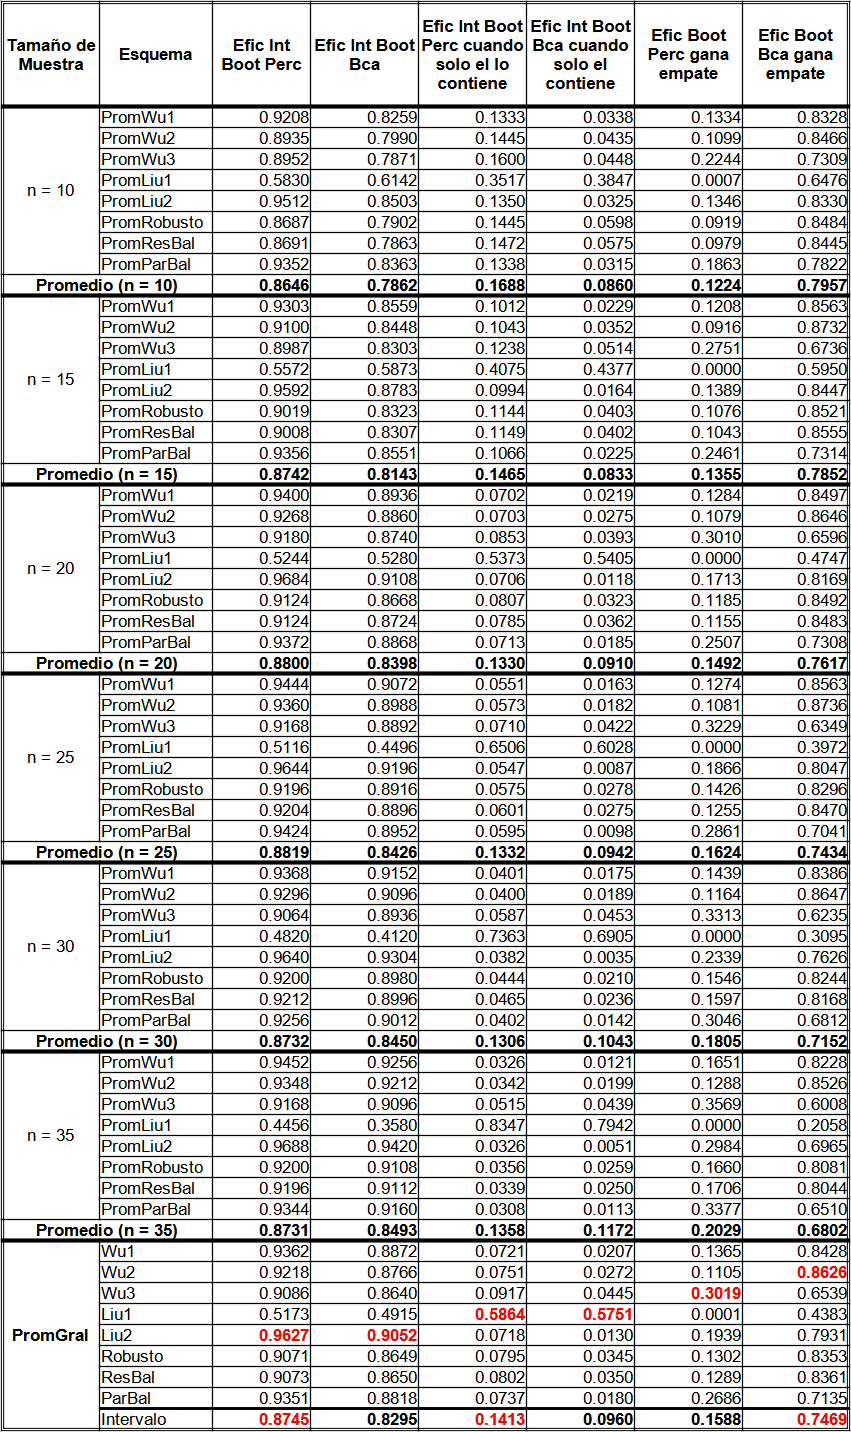
\includegraphics[width=0.55\linewidth]{img/EI_NVC_Efic_Boots.png} 
	\caption{Eficiencia promedio de los intervalos Bootstrap por tamaño de muestra y esquema de remuestreos para el caso EI-NVC.} 
	\label{fig:EficPromIntBootsTamMuestEsqRemuEI-NVC}
\end{figure}
\FloatBarrier


\begin{figure}[ht] 
	\centering 
	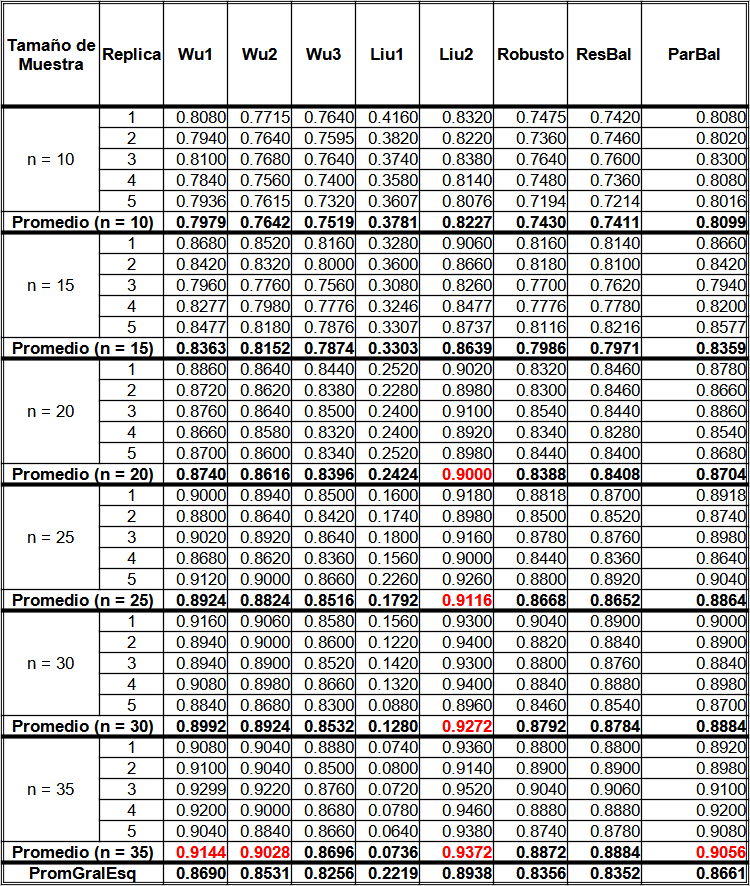
\includegraphics[width=0.70\linewidth]{img/EI_NVC_Efic_Esq.png} 
	\caption{Eficiencia promedio de los esquemas por tamaño de muestra y esquema de remuestreos para el caso EI-NVC.} 
	\label{fig:EficPromEsqTamMuesEsqRemuEI-NVC}
\end{figure}
\FloatBarrier


\textbf{EI-NNVC}\\

\begin{figure}[ht] 
	\centering 
	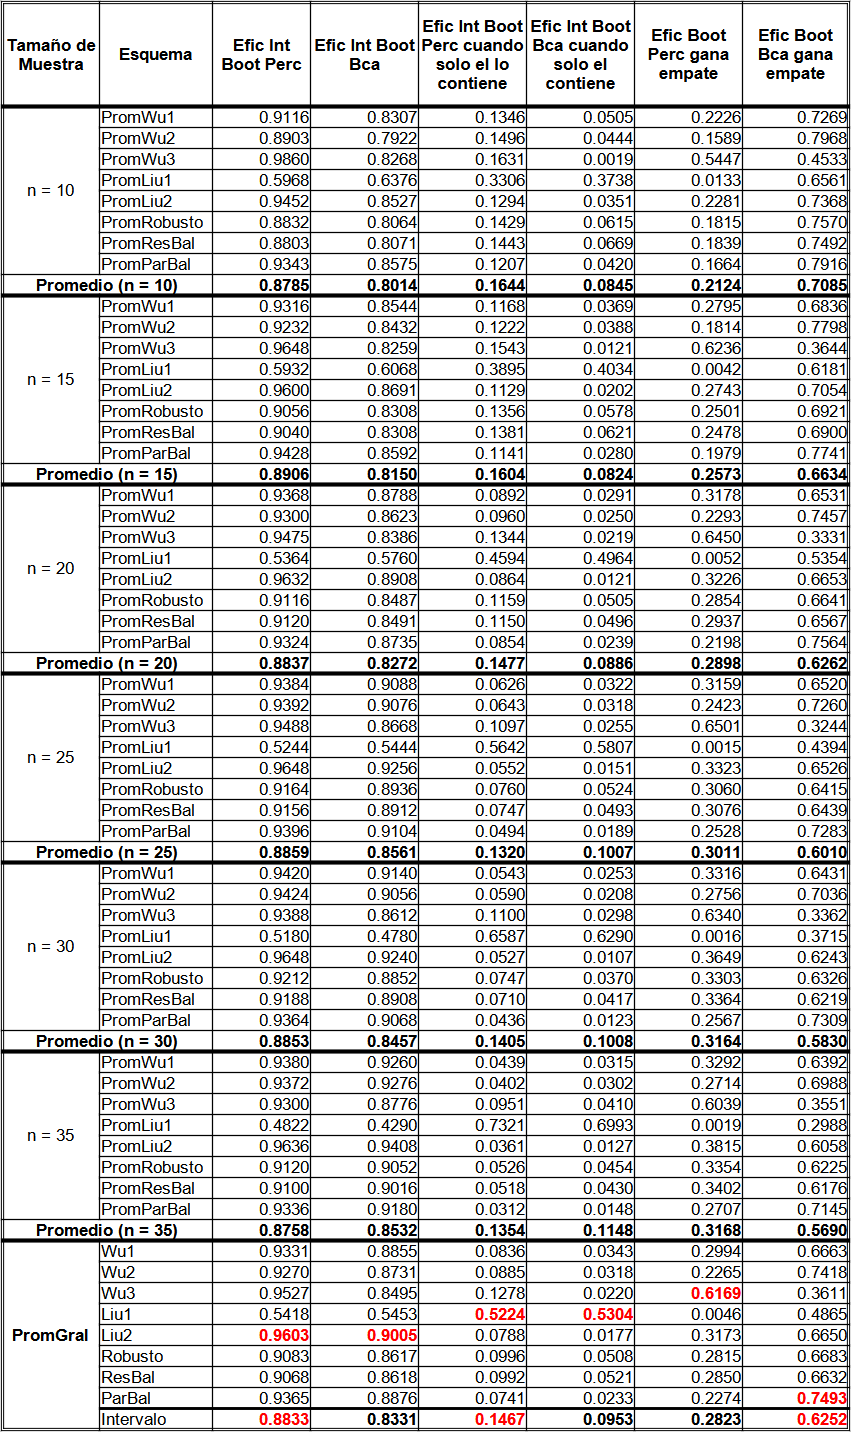
\includegraphics[width=0.55\linewidth]{img/EI_NNVC_Efic_Boots.png} 
	\caption{Eficiencia promedio de los intervalos Bootstrap por tamaño de muestra y esquema de remuestreos para el caso EI-NNVC.} 
	\label{fig:EficPromIntBootsTamMuestEsqRemuEI-NNVC}
\end{figure}
\FloatBarrier



\begin{figure}[ht] 
	\centering 
	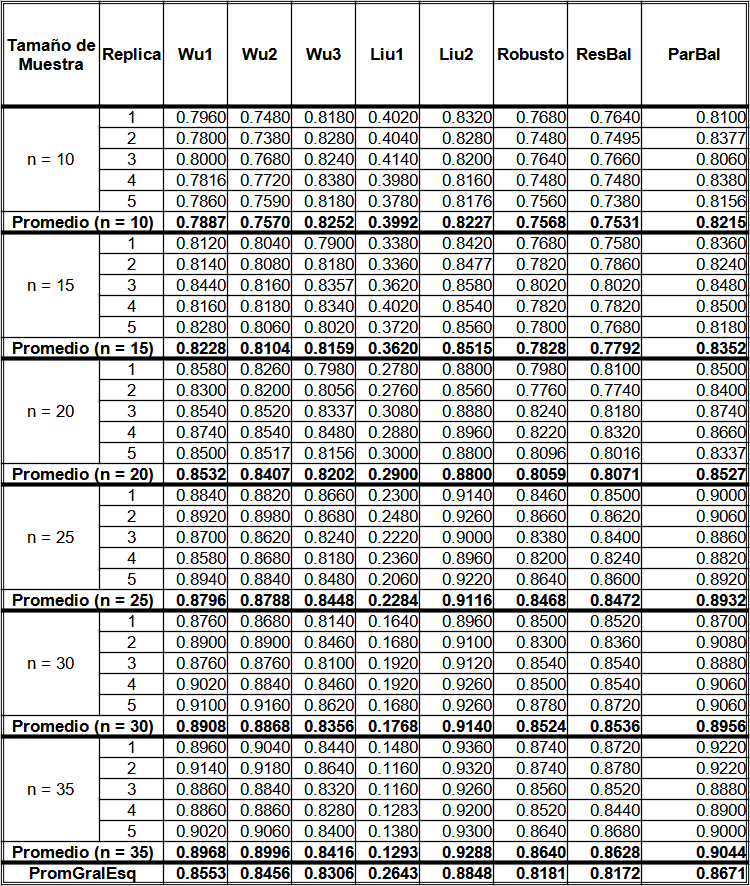
\includegraphics[width=0.70\linewidth]{img/EI_NNVC_Efic_Esq.png} 
	\caption{Eficiencia promedio de los esquemas por tamaño de muestra y esquema de remuestreos para el caso EI-NNVC.} 
	\label{fig:EficPromEsqTamMuesEsqRemuEI-NNVC}
\end{figure}
\FloatBarrier



\textbf{EI-NVD}\\

\begin{figure}[ht] 
	\centering 
	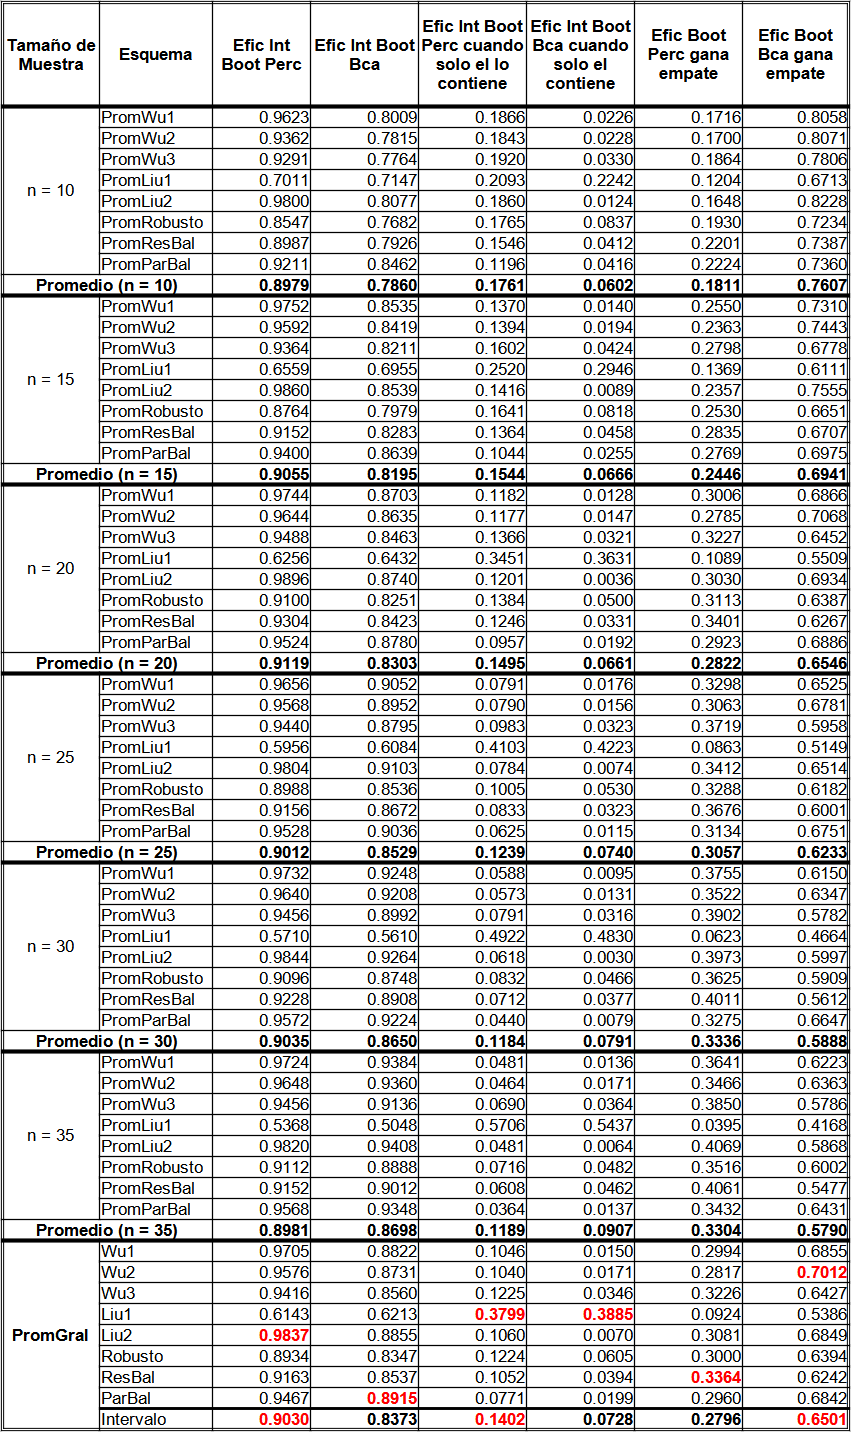
\includegraphics[width=0.55\linewidth]{img/EI_NVD_Efic_Boots.png} 
	\caption{Eficiencia promedio de los intervalos Bootstrap por tamaño de muestra y esquema de remuestreos para el caso EI-NVD.} 
	\label{fig:EficPromIntBootsTamMuestEsqRemuEI-NVD}
\end{figure}
\FloatBarrier


\begin{figure}[ht] 
	\centering 
	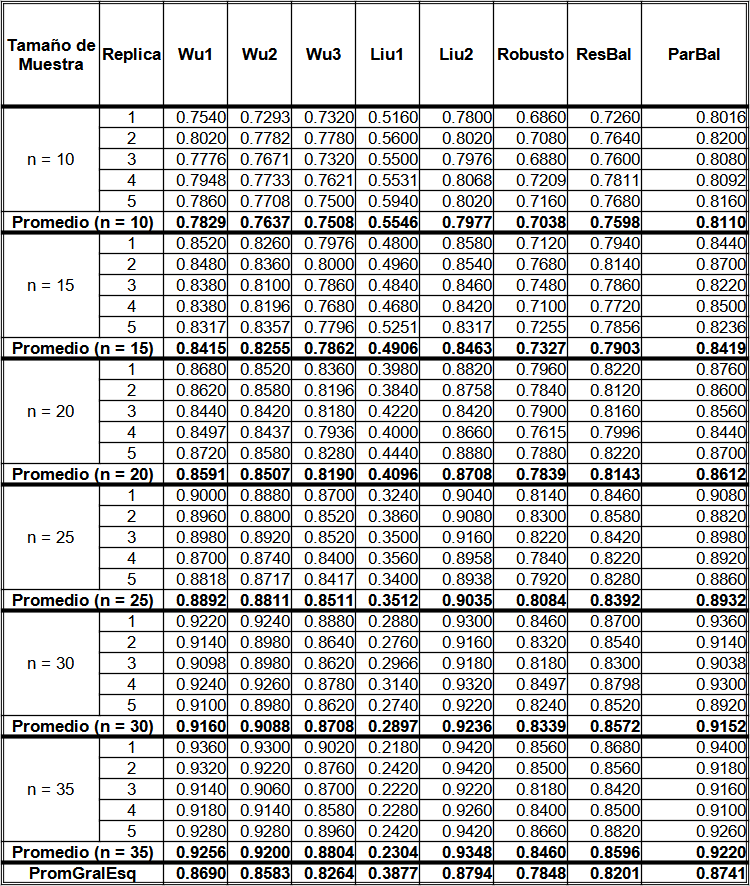
\includegraphics[width=0.70\linewidth]{img/EI_NVD_Efic_Esq.png} 
	\caption{Eficiencia promedio de los esquemas por tamaño de muestra y esquema de remuestreos para el caso EI-NVD.} 
	\label{fig:EficPromEsqTamMuesEsqRemuEI-NVD}
\end{figure}
\FloatBarrier




\textbf{EI-NNVD}\\

\begin{figure}[ht] 
	\centering 
	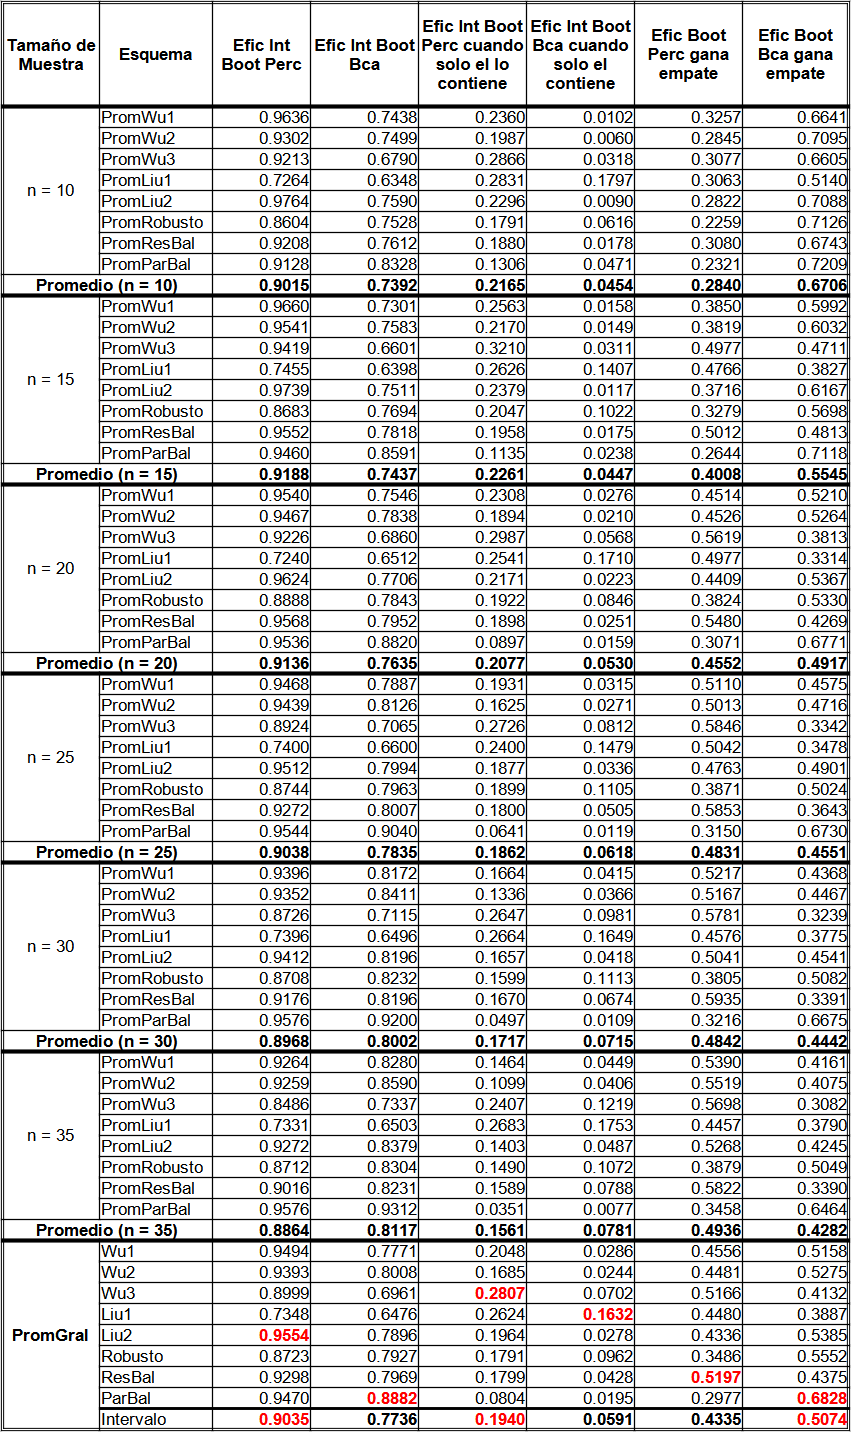
\includegraphics[width=0.55\linewidth]{img/EI_NNVD_Efic_Boots.png} 
	\caption{Eficiencia promedio de los intervalos Bootstrap por tamaño de muestra y esquema de remuestreos para el caso EI-NNVD.} 
	\label{fig:EficPromIntBootsTamMuestEsqRemuEI-NNVD}
\end{figure}
\FloatBarrier




\begin{figure}[ht] 
	\centering 
	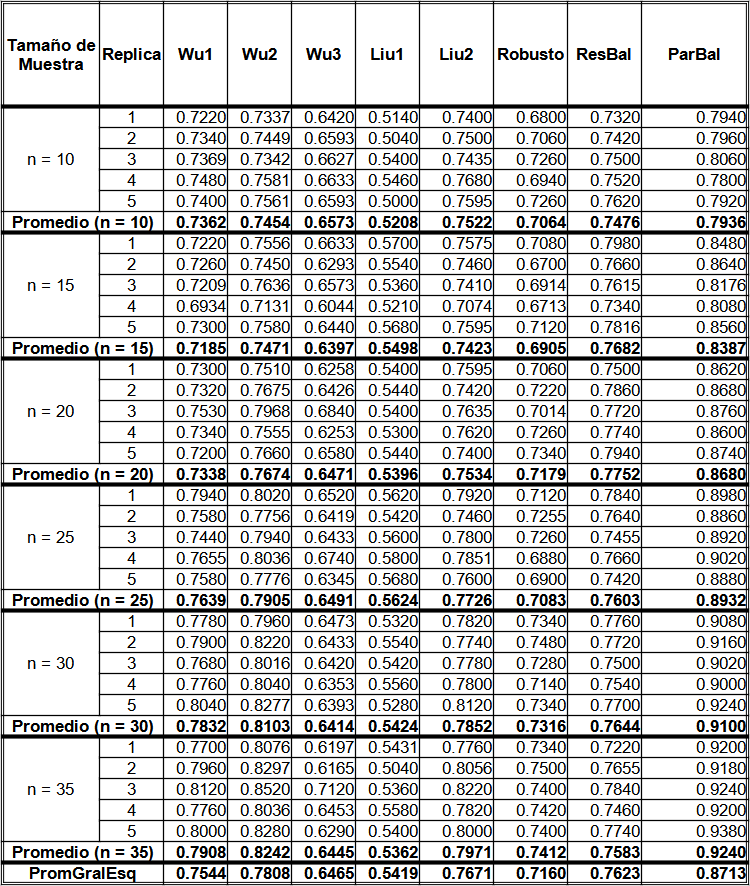
\includegraphics[width=0.70\linewidth]{img/EI_NNVD_Efic_Esq.png} 
	\caption{Eficiencia promedio de los esquemas por tamaño de muestra y esquema de remuestreos para el caso EI-NNVD.} 
	\label{fig:EficPromEsqTamMuesEsqRemuEI-NNVD}
\end{figure}
\FloatBarrier


\textbf{Para todos los supuestos para el caso EI}

\begin{figure}[ht] 
	\centering 
	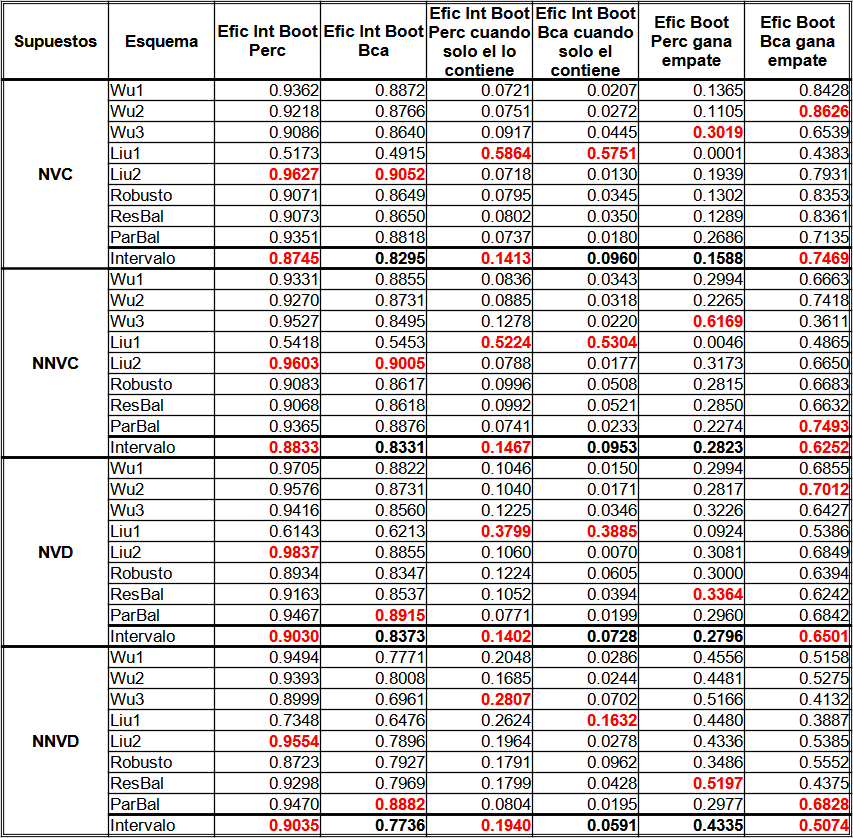
\includegraphics[width=0.80\linewidth]{img/EI_Prom_Supuestos.png} 
	\caption{Promedio de supuestos utilizados para el caso EI.} 
	\label{fig:PromSupuUtiliEI}
\end{figure}
